
\paragraph{Real-world setup.} 
We evaluate WAV on a real-world dual-arm robotic platform, Piper, across a set of challenging manipulation tasks designed to probe key policy capabilities, including spatial reasoning, deformable object manipulation, visual grounding, and long-horizon planning. 
Representative tasks include \textbf{bowl organization}, \textbf{towel flattening}, and a \textbf{long-horizon drawer task} that requires opening a drawer, placing an object inside, and closing it.

For a fair comparison, we select GE-ACT~\citep{liao2025genie} as the baseline model, as it uses the same video pre-trained model and has a similar network architecture and parameter count.
Following standard practice, we adopt a strict binary success metric: a trial is considered successful only if the task is fully completed, with no partial credit. 
More details are in Appendix Sec.~\ref{appendix:Implementation_Details}.

\begin{wrapfigure}{r}{0.5\textwidth}
    \centering
    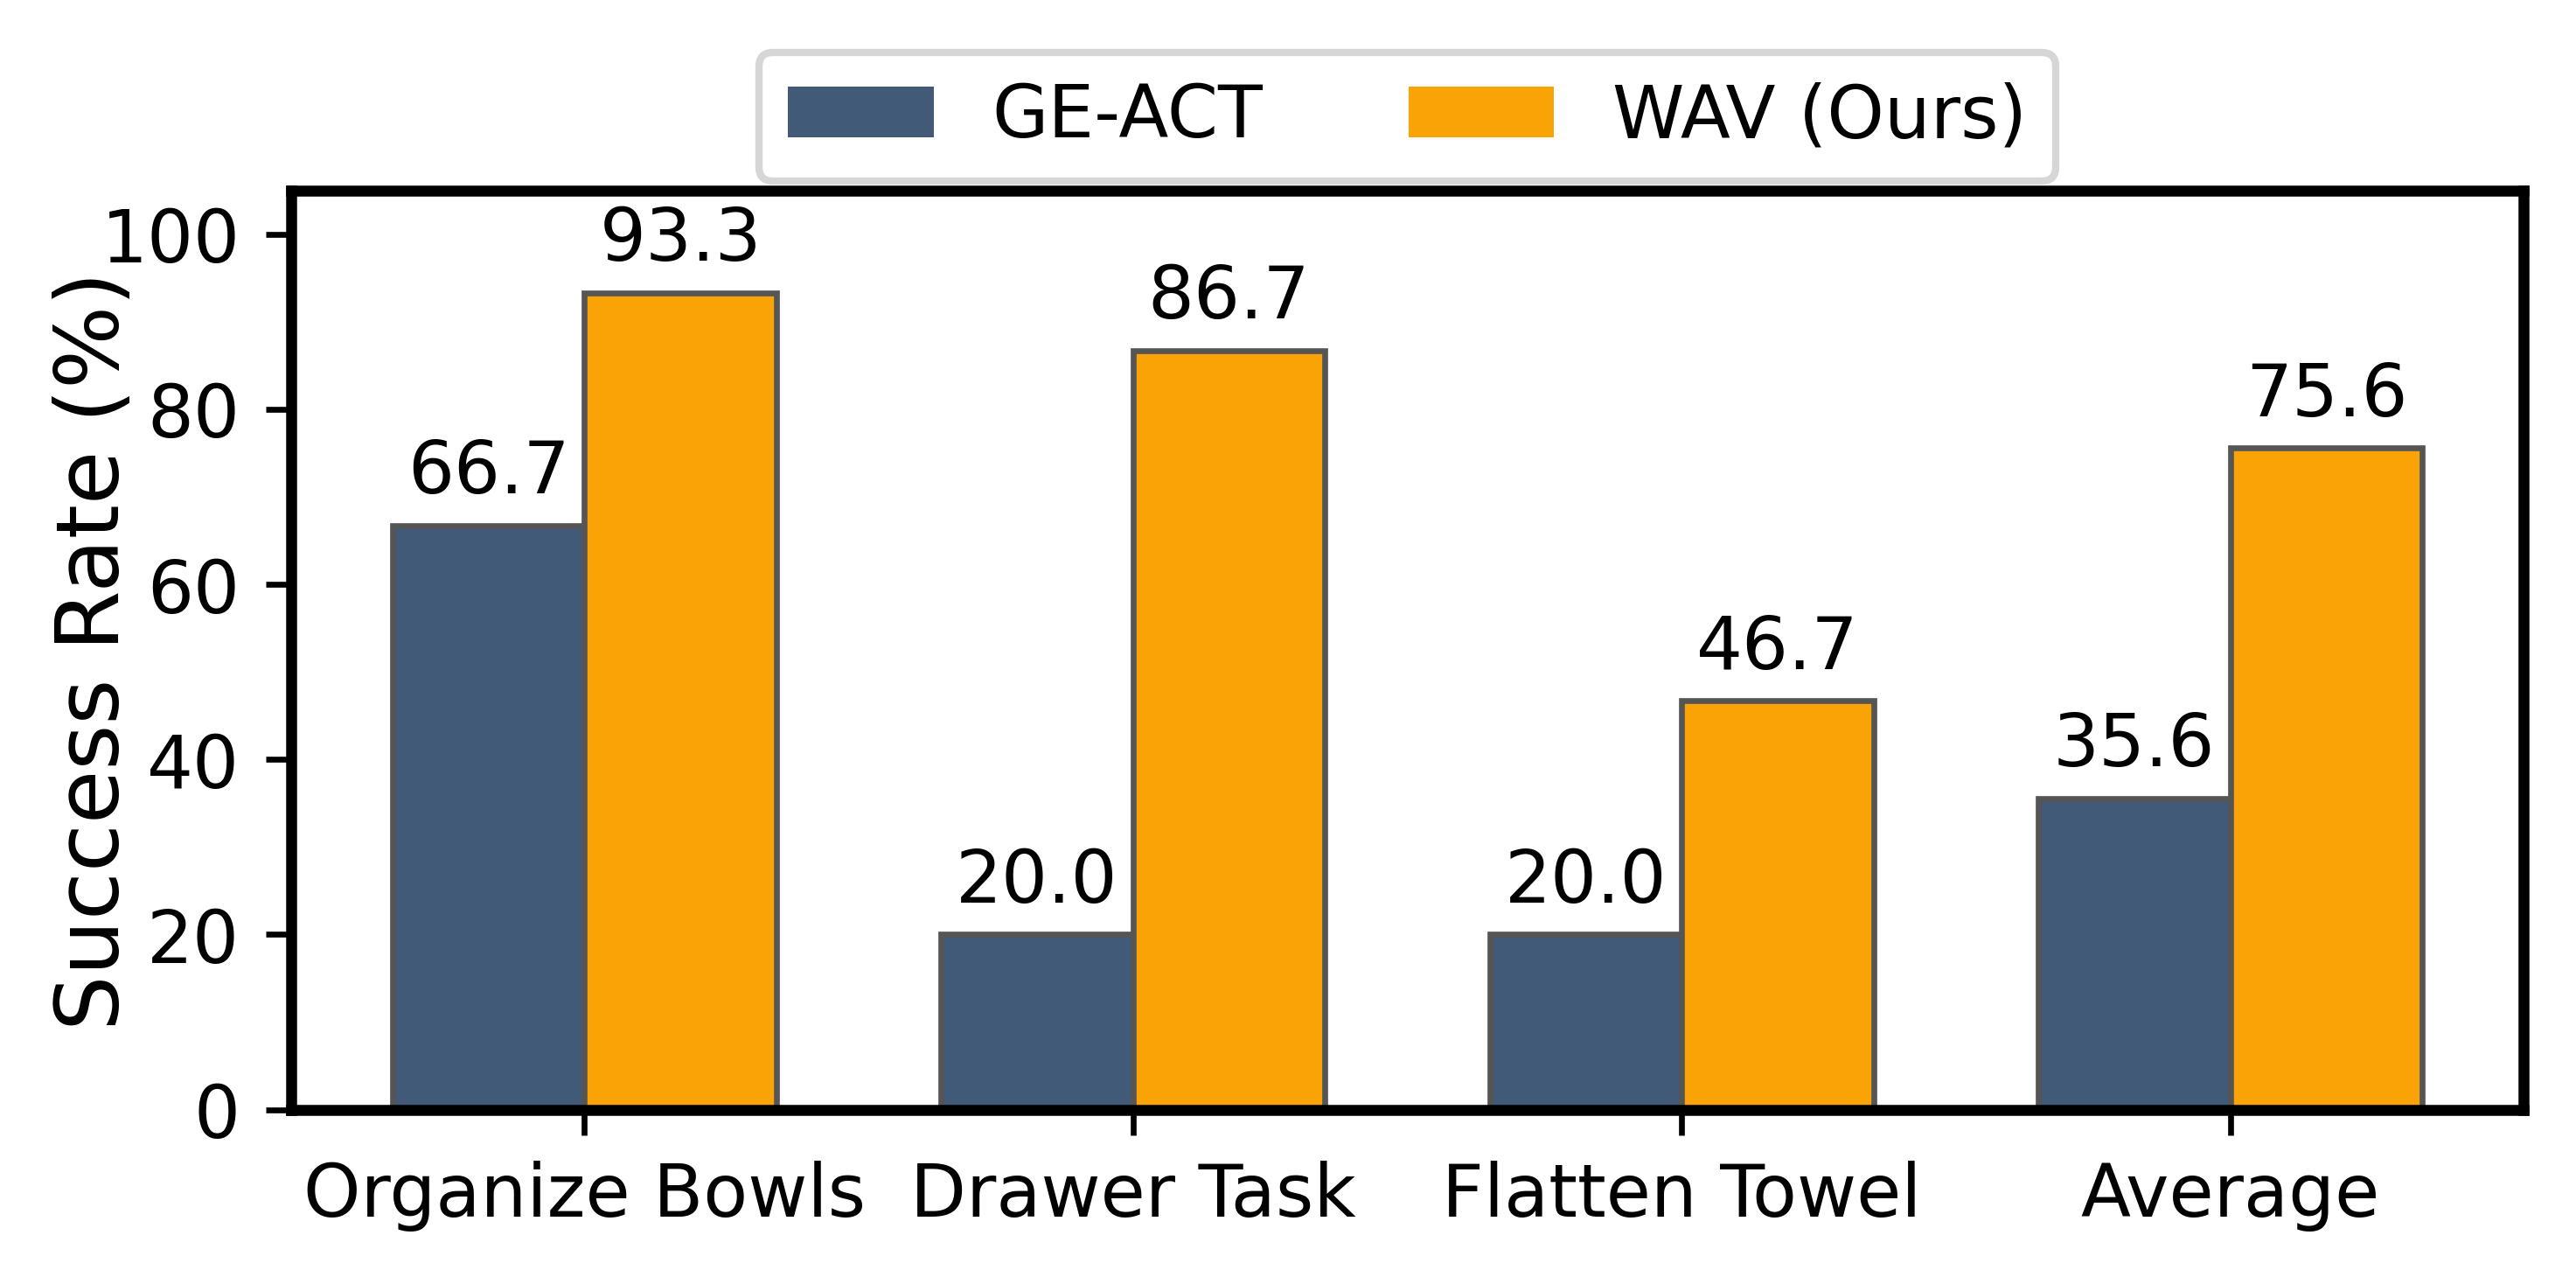
\includegraphics[width=1\linewidth]{figures/real_world_bar.png}
    \caption{
    Quantitative comparison between WAV model (Ours) and the GE-ACT (Baseline) on real-world tasks. 
    Each result is averaged over 15 trials.
    }
    \label{fig:real_world_bar}
\end{wrapfigure}
\paragraph{Results.} 

As shown in Fig.~\ref{fig:real_world_bar}, WAV achieved a significantly higher success rate across all tasks than the baseline, with the average success rate increasing from 35.6\% to 75.6\%.

Qualitative results (Fig.~\ref{fig:real_world_tasks}) reveal distinct failure modes of the baseline. 
GE-ACT frequently exhibits inaccurate action execution and weak spatial grounding, such as misaligning with the drawer handle or failing to grasp objects reliably. 
These errors accumulate over multiple steps, leading to cascading failures in long-horizon tasks. 
In contrast, WAV produces more consistent and coherent multi-step behaviors. 
By implicitly planning over future trajectories, it anticipates downstream consequences of actions, resulting in more accurate interactions and improved robustness. 
This advantage is most pronounced in tasks requiring multi-step coordination, highlighting the role of implicit planning in mitigating error accumulation in real-world settings.

\begin{figure}[htbp]
\centering
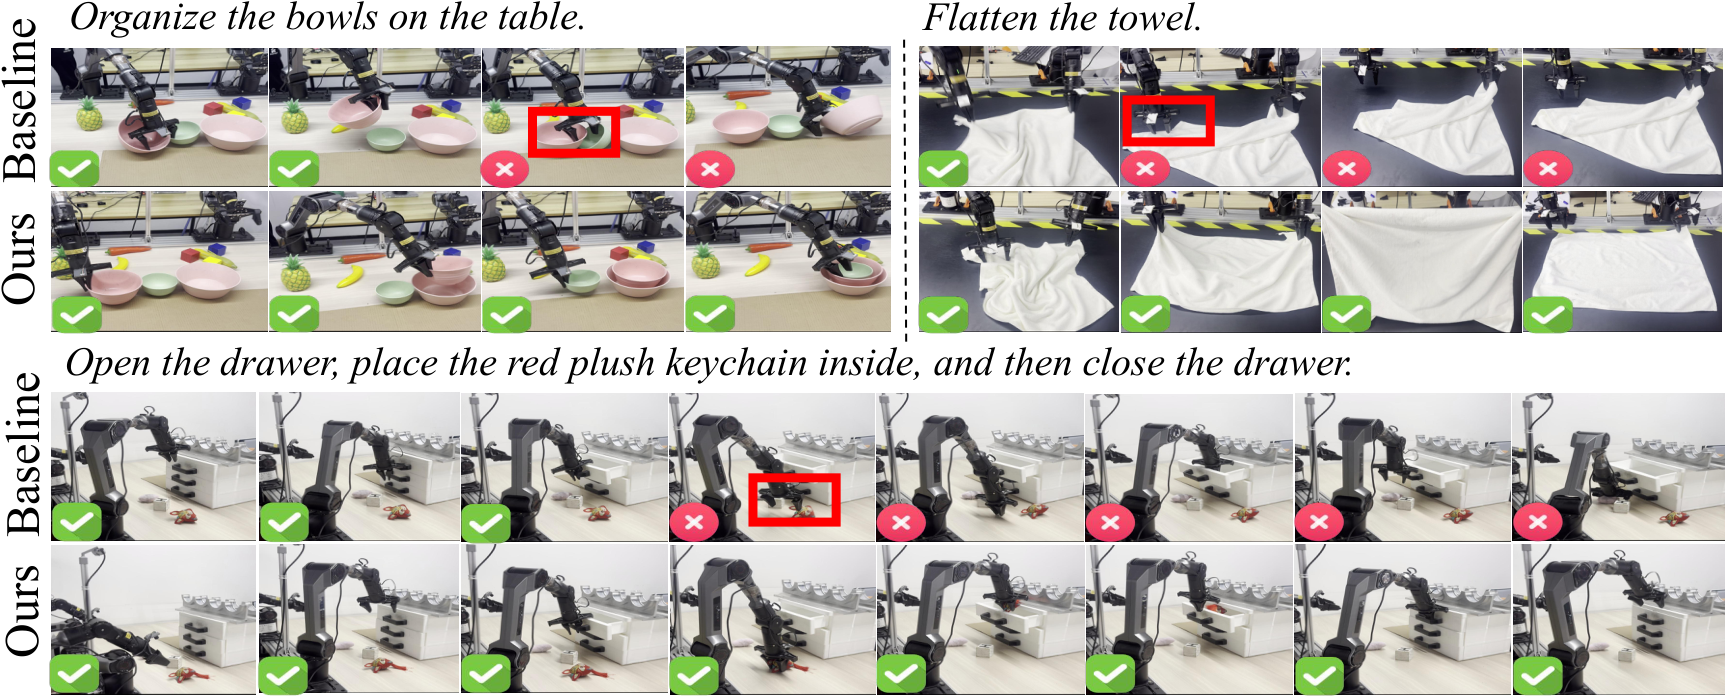
\includegraphics[width=\textwidth]{figures/real_world_tasks.pdf}
\caption{
Qualitative comparison between WAV model (Ours) and the GE-ACT (Baseline) across different real-world manipulation tasks. 
}
  \label{fig:real_world_tasks}
\end{figure}

